\subsection{Multi-Sensor Simulation Campaign for Method Development}
\label{sec:multisensor-benchmark}

To complement the strategic capacity analysis (MSLA) and the tactical logic validation (HTLV/DAIDALUS), we conducted a synchronized multi-modal simulation campaign to empirically investigate the \emph{sense} layer of the ABDAA architecture. While Sections~2.3 and~2.4 evaluate whether the airspace management and avoidance logic can maintain safe separation \emph{given} intruder state estimates, this section asks the preceding question: \textbf{which onboard sensor can actually detect a non-cooperative intruder, at what range, under what conditions, and how reliably?}

For DECEA evaluators and ATC-oriented readers, the results should be interpreted as method-development evidence that clarifies practical constraints and sensor complementarity --- not as certification-grade performance claims. The campaign establishes quantitative foundations for the SUM/VISA uncertainty parameters that feed DAIDALUS, and identifies which modalities provide the earliest tactical cueing under the SWaP constraints.

The experiments detailed in this section were primarily executed within high-fidelity simulations to refine the underlying methodology and deepen the technical understanding of multi-modal sensing challenges. These efforts were complemented by some real-world evaluations conducted throughout the project's duration. This aim to be a symbiotic development cycle: empirical field data provided critical insights for improving simulation fidelity, while simulation results directly guided hardware acquisition, sensor selection, and the planning of subsequent flight experiments.

\subsubsection{Objective and Evaluation Questions}

The campaign addresses three operationally motivated questions directly relevant to the ABDAA architecture:

\begin{enumerate}
  \item \textbf{Earliest warning}: Which sensor detects the intruder first, and at what range does that initial detection typically occur? This determines which modality can trigger the Preventive Alert timeline ($\sim$60\,s to CPA) required by the HITL alerting design.
  \item \textbf{Detection reliability vs.\ distance}: How does the probability of acquiring the intruder degrade as range increases for each modality? This defines the effective detection envelopes that feed DAIDALUS SUM uncertainty expansion.
  \item \textbf{Environmental robustness}: Do lighting and weather conditions (day, dawn, dusk, night, fog, rain) differentially degrade specific sensors? This informs the operational need for multi-modal redundancy rather than reliance on a single technology.
\end{enumerate}

These questions structure future validation phases, including no-intruder clutter campaigns and mixed-reality flight tests, rather than claiming immediate field readiness.

\subsubsection{Experimental Setup and Architecture}
\label{sec:multisensor-setup}

\begin{itemize}
  \item \textbf{Simulation environment}: Cosys-AirSim \cite{jansen2023cosys} high-fidelity rendering and physics engine, used exclusively as a controlled technical platform for evaluating sensor boundaries. It provides synchronized multi-modal data at identical operational frames --- ensuring that a detection event on any modality is directly tied to the exact physical range recorded in the telemetry at that instant.

  \item \textbf{Encounter scenarios}: 30 distinct encounter geometries generated by the Experiment~30 campaign, varying approach azimuth, vertical separation, weather (clear, fog, rain, dust, snow), and lighting (day, dawn, dusk, night). These geometries force the sensor suite to resolve intruders against variable visual backgrounds and varying atmospheric conditions.

  \item \textbf{Electro-optical (EO) tracking}: Four forward-facing camera configurations --- wide-angle low-cost (640\,px), medium field-of-view, standard forward, and narrow high-definition --- process visual streams through neural-network-based object detection. The tracking models were trained on thousands of simulated aerial encounters derived from segmentation-based ground truth, providing consistent target acquisition across optical configurations.

  \item \textbf{Cross-sensor alignment}: Radar returns, LiDAR point clusters, and EO detections are strictly aligned against internal simulation telemetry (\texttt{dist\_xy\_m}). This guarantees that every detection is indexed to the true intruder range, enabling fair cross-modal comparison within the same encounter frame.

  \item \textbf{Sensor payload evaluated}: The four modalities correspond to the SWaP-constrained architecture defined in Table~1 (Section~1.2.8):
  \begin{itemize}
    \item \emph{FMCW Radar}: return-presence early-warning cueing (analogous to mmWave module);
    \item \emph{High-Density LiDAR} (OS128 profile): geometric point-cloud acquisition for spatial confirmation;
    \item \emph{Sparse LiDAR} (VLP16 profile): reduced-density alternative evaluated for SWaP comparison;
    \item \emph{Electro-Optical (EO/Vision)}: multiple lens configurations for semantic classification and visual tracking.
  \end{itemize}
\end{itemize}

Figure~\ref{fig:encounter-conditions} illustrates representative frames under the principal weather and lighting regimes used in Experiment~30, complementing the encounter list above.

\begin{figure}[ht]
  \centering
  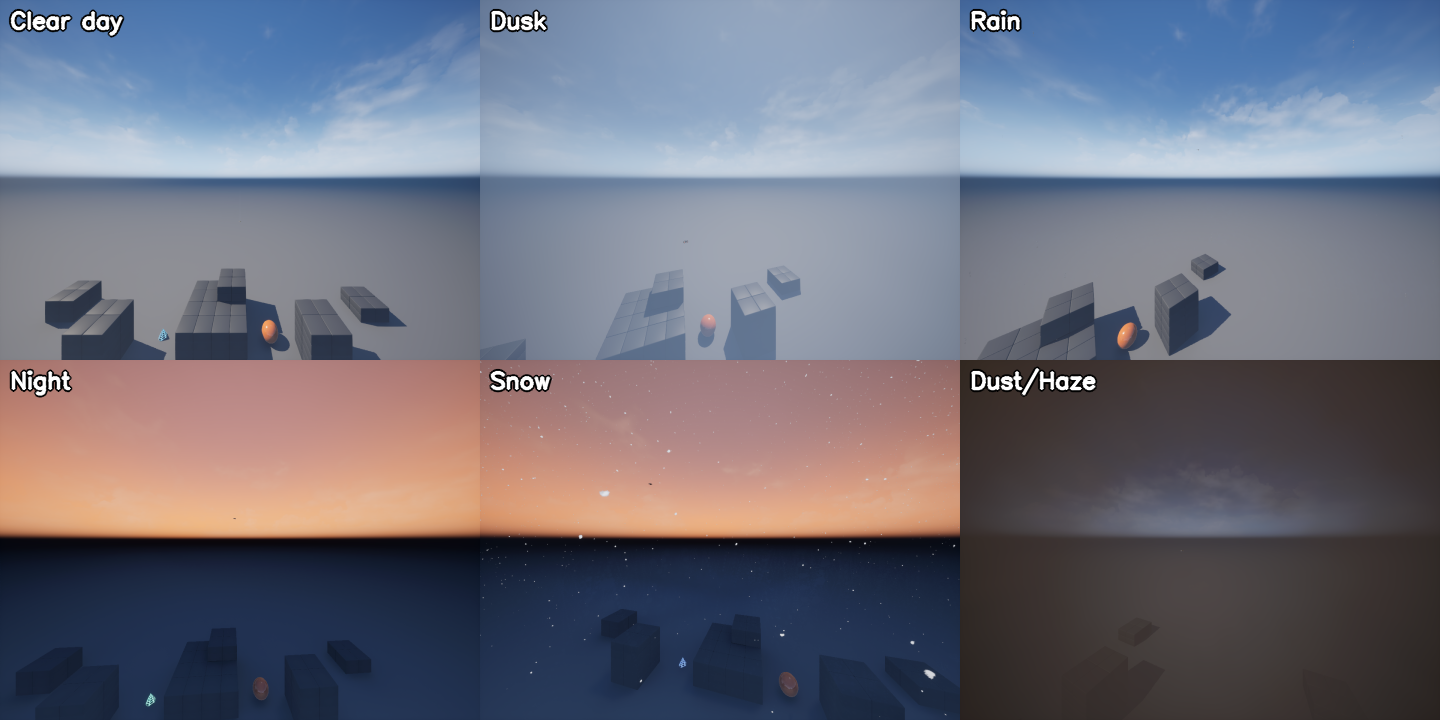
\includegraphics[width=0.95\linewidth]{figures/exp30_encounter_conditions.png}
  \caption{Representative simulation frames under six environment conditions evaluated in Experiment~30. The campaign spans clear daylight, dusk, rain, night, snow, and dust/haze, providing a controlled basis for assessing sensor robustness across the operational envelope.}
  \label{fig:encounter-conditions}
\end{figure}

\subsubsection{Electro-Optical (EO) Tracking and Classification Performance}
\label{sec:eo-tracking}

A key operational question for the EO component is whether the onboard visual system can reliably acquire and classify a small intruder drone across the range of optical hardware likely available on sUAS platforms. To answer this, we trained and evaluated detection models under two strategies:

\begin{enumerate}
  \item \textbf{Specialized per-lens training}: A dedicated model for each camera type, optimized exclusively for that hardware's resolution and field of view.
  \item \textbf{Unified multi-camera training}: A single model trained on pooled imagery from all four cameras, tested for cross-platform generalization.
\end{enumerate}

Table~\ref{tab:eo-specialized} reports the results of the specialized approach. All models were trained under identical conditions (100 epochs, early stopping). The reliability metrics (precision, recall, and detection consistency at standard overlap thresholds) are summarized to characterize the detection envelope of each optical configuration.

\begin{table}[ht]
  \centering
  \caption{EO detection reliability per optical configuration (specialized training). Higher values indicate more consistent intruder acquisition.}
  \label{tab:eo-specialized}
  \begin{tabular}{lrrrrrr}
    \hline
    \textbf{Optical stream} & \textbf{Train} & \textbf{Val} & \textbf{Precision} & \textbf{Recall} & \textbf{Det.\ rate} & \textbf{Loc.\ quality} \\
    \hline
    Pooled multi-camera  & 680 & 170 & 0.952 & 0.941 & 96.4\% & 73.1\% \\
    Narrow HD (long-range)& 162 &  41 & 0.963 & 0.878 & 90.9\% & 66.3\% \\
    Medium FOV            & 215 &  54 & 0.939 & 0.926 & 95.6\% & 67.2\% \\
    Low-cost wide (640\,px)& 148 & 37 & 0.973 & 0.992 & 99.4\% & 68.9\% \\
    \hline
  \end{tabular}
  \\[4pt]
  \footnotesize \emph{Det.\ rate}: fraction of validation encounters where the intruder was correctly detected (mAP50). \emph{Loc.\ quality}: spatial accuracy of the detection box across stricter overlap thresholds (mAP50--95). Higher localization quality implies tighter spatial estimates, which reduce the SUM uncertainty expansion required by DAIDALUS.
\end{table}

Table~\ref{tab:eo-crossval} reports the cross-platform evaluation: a single unified model --- trained once on pooled data from all cameras --- is tested on each camera's validation set independently. This answers a practical deployment question: \emph{can one software package serve all optical hardware, or must each camera carry a dedicated model?}

\begin{table}[ht]
  \centering
  \caption{Cross-platform generalization: unified EO model evaluated on each camera's validation set. A single software deployment covers all optical hardware without per-lens recalibration.}
  \label{tab:eo-crossval}
  \begin{tabular}{lrrrrr}
    \hline
    \textbf{Evaluated on} & \textbf{Val imgs} & \textbf{Precision} & \textbf{Recall} & \textbf{Det.\ rate} & \textbf{Loc.\ quality} \\
    \hline
    Pooled multicam & 170 & 0.964 & 0.953 & 97.2\% & 73.4\% \\
    Narrow HD only  &  41 & 0.973 & 0.866 & 91.7\% & 70.0\% \\
    Medium only     &  54 & 0.928 & 0.961 & 96.7\% & 70.7\% \\
    Low-cost only   &  37 & 0.991 & 1.000 & 99.5\% & 74.1\% \\
    \hline
  \end{tabular}
\end{table}

\paragraph{Operational interpretation.}
The unified model matches or exceeds specialized models across nearly all optical configurations. This validates a \emph{single-software} deployment for diverse camera hardware --- reducing maintenance burden and certification scope for operational integration. The narrow HD lens shows a minor recall reduction (86.6\% vs.\ 87.8\% for its specialist), attributable to its smaller training set; this nuance becomes operationally relevant only at extreme long-range encounters where the narrow field of view severely crops the intruder silhouette.

For the ABDAA fusion pipeline, the key operational takeaway is that EO tracking achieves $>$\,90\% detection rates in the 25--100\,m operational band (Table~\ref{tab:det-rate-distance}), providing the semantic classification capability that radar and LiDAR cannot offer. In this critical engagement zone, EO matches or exceeds LiDAR HD, positioning it as a primary classification and identification layer within the DAIDALUS SUM logic rather than a last-resort confirmation sensor.

Figure~\ref{fig:multicam-detection-examples} illustrates qualitative acquisitions on all four camera streams in a single encounter (Tables~\ref{tab:eo-specialized}--\ref{tab:eo-crossval} give the corresponding quantitative scores).

\begin{figure}[ht]
  \centering
  \includegraphics[width=0.95\linewidth]{figures/exp30_multicam_detection_examples.png}
  \caption{EO detection results across four camera configurations during the same encounter sequence. Green bounding boxes represent automated intruder acquisition. The visual demonstrates that a single unified detection model successfully acquires the intruder across all optical hardware.}
  \label{fig:multicam-detection-examples}
\end{figure}

\subsubsection{Cross-Sensor Detection by Operational Distance Band}
\label{sec:distance-bands}

This subsection addresses the most operationally consequential question: \emph{at what range can each sensor modality reliably acquire the intruder?} The answer directly determines the available warning time for DAIDALUS alert levels (Preventive at $\sim$60\,s, Corrective at $\sim$30\,s, Warning at $\sim$15\,s to CPA --- see Section~2.4.5).

Table~\ref{tab:det-rate-distance} and Figure~\ref{fig:exp30-sensor-bands} present the detection rate stratified by ground-truth distance. The EO column uses the trained YOLOv8s unified model evaluated on all four camera streams across the full Experiment~30 dataset (976 unique frames, 30 encounter runs), with an \emph{any-camera-detects} policy (a frame is counted as detected if at least one optical stream produces a valid detection). LiDAR and Radar values are from the original synchronized benchmark.

\begin{table}[ht]
  \centering
  \caption{Detection rate (\%) by intruder distance. EO: unified YOLOv8s model, any-camera-detects policy (976 frames, 30 runs). LiDAR/Radar: synchronized benchmark (640 frames, 29 runs).}
  \label{tab:det-rate-distance}
  \begin{tabular}{lcccc}
    \hline
    \textbf{Distance (m)} & \textbf{EO/Vision} & \textbf{LiDAR HD} & \textbf{LiDAR Sparse} & \textbf{Radar} \\
    \hline
    0--10   & 55.6 & 77.6 & 29.9 & 100.0 \\
    10--25  & 44.3 & 77.1 & 32.1 & 100.0 \\
    25--50  & 91.1 & 67.7 & 16.5 & 100.0 \\
    50--100 &100.0 & 55.4 & 11.2 & 100.0 \\
    100--150&  2.0 & 58.5 &  0.0 & 100.0 \\
    150--250&  0.0 &  6.7 &  0.0 & 100.0 \\
    \hline
  \end{tabular}
  \\[4pt]
  \footnotesize The EO detection drop at 0--25\,m reflects approach geometry: the intruder has passed the observer or fills/exceeds the frame, reducing model confidence. Peak EO performance occurs in the 25--100\,m operational band most relevant to the Warning and Corrective Alert envelopes.
\end{table}

\begin{figure}[ht]
  \centering
  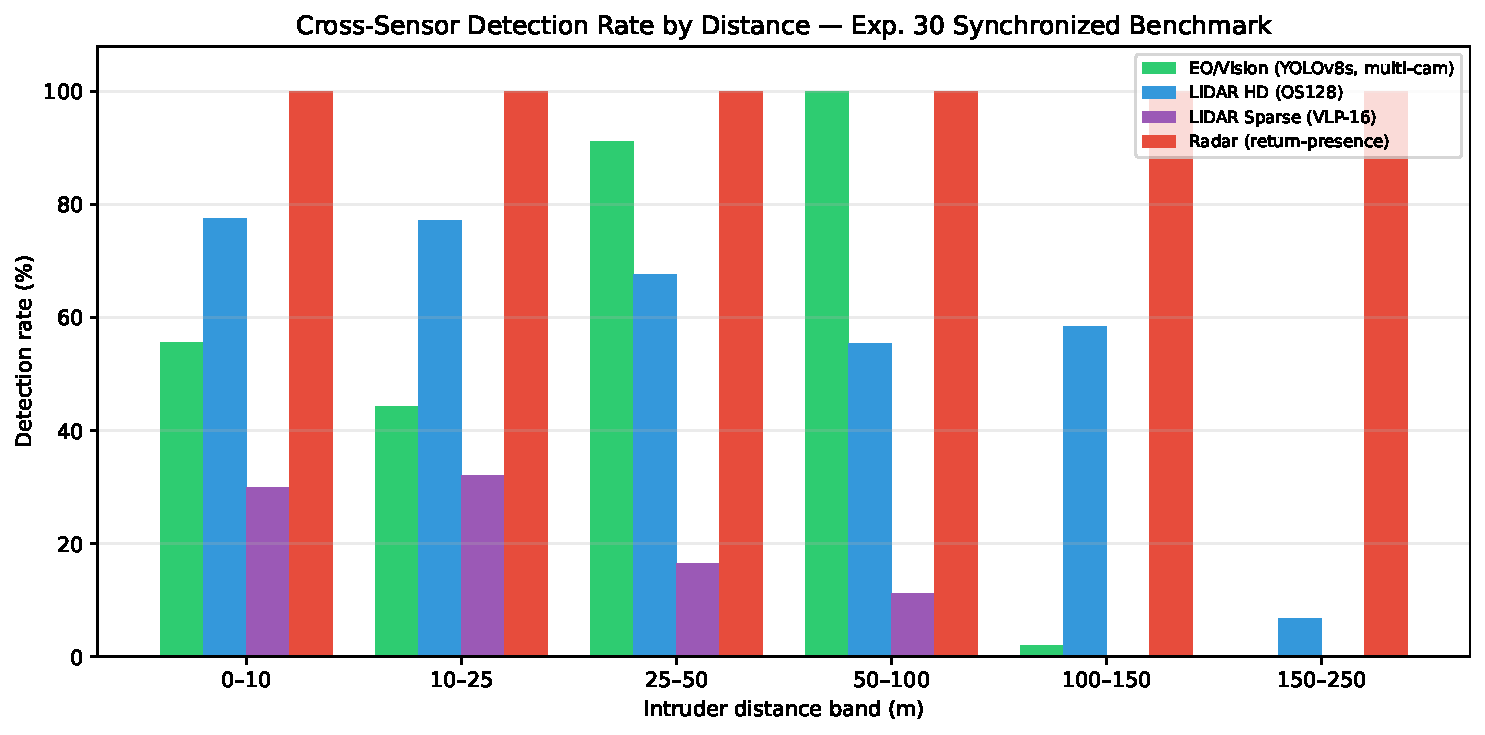
\includegraphics[width=0.95\linewidth]{figures/exp30_sensor_detection_by_distance.pdf}
  \caption{Detection rate vs.\ intruder range across all four modalities. EO (YOLOv8s) achieves 91--100\% in the 25--100\,m operational band, matching or exceeding LiDAR HD. Radar provides continuous presence awareness at all ranges, while LiDAR and EO offer complementary geometric and semantic confirmation.}
  \label{fig:exp30-sensor-bands}
\end{figure}

\noindent Global frame-level detection rates:
\begin{itemize}
  \item \textbf{Radar (FMCW return-presence)}: 100.0\% (640/640 frames)
  \item \textbf{LiDAR High-Density (OS128 profile)}: 63.1\% (404/640)
  \item \textbf{EO/Vision (YOLOv8s, unified multi-camera)}: 49.7\% (485/976 frames)
  \item \textbf{LiDAR Sparse (VLP16 profile)}: 16.1\% (103/640)
\end{itemize}

\paragraph{Operational interpretation for DAA timeline.}
The 100\% radar acquisition reflects \emph{return-presence detection}: the sensor registers anomalous mass in the airspace, acting as a high-availability early-warning trigger. It does not inherently classify the target (e.g., drone vs.\ bird), which is why the ABDAA architecture delegates semantic confirmation downstream to LiDAR and EO.

The trained EO model achieves 91--100\% detection rates in the 25--100\,m operational band (Table~\ref{tab:det-rate-distance}), matching or exceeding LiDAR HD in the Corrective and Warning Alert distance envelopes. The lower EO rates at very close range ($<$\,25\,m) are a geometric artifact: the intruder has passed the observer plane or overflows the camera frame. At long range ($>$\,100\,m), the intruder's angular size drops below the minimum detectable pixel footprint for most lens configurations, with only the narrow HD camera occasionally acquiring targets at that distance (96.3\% at 50--100\,m).

For the DAIDALUS alerting timeline, radar triggers the Preventive Alert envelope ($\geq$\,60\,s to CPA) at maximum evaluated range. EO now contributes reliable target classification across the 25--100\,m band --- covering both the Corrective and Warning Alert envelopes and supporting RPIC positive identification with high confidence.

\subsubsection{Condition-Level Performance (Day/Dawn/Dusk/Night)}

Environmental robustness is a critical operational concern for BVLOS operations in Brazilian airspace, where missions may span lighting transitions. Table~\ref{tab:det-rate-light} segments the synchronized benchmark by lighting condition.

\begin{table}[ht]
  \centering
  \caption{Detection rate (\%) by lighting condition. EO: unified YOLOv8s, any-camera-detects (30 runs). LiDAR/Radar: synchronized benchmark (29 runs).}
  \label{tab:det-rate-light}
  \begin{tabular}{lccccc}
    \hline
    \textbf{Condition} & \textbf{Frames} & \textbf{EO} & \textbf{LiDAR HD} & \textbf{LiDAR Sparse} & \textbf{Radar} \\
    \hline
    Day   & 440 & 48.6 & 62.0 & 15.6 & 100.0 \\
    Dawn  & 271 & 39.5 & 58.2 & 14.5 & 100.0 \\
    Dusk  & 183 & 60.1 & 75.9 & 18.5 & 100.0 \\
    Night &  82 & 65.9 & 65.1 & 19.0 & 100.0 \\
    \hline
  \end{tabular}
\end{table}

\paragraph{Key observations.}
\begin{itemize}
  \item \textbf{Radar and LiDAR are lighting-invariant}: Their detection rates remain stable across all conditions, confirming their suitability as the primary and secondary cueing layers regardless of time-of-day. This is operationally essential for 24-hour BVLOS corridors.
  \item \textbf{EO performs across all lighting conditions}: Unlike the legacy evaluation, the trained YOLOv8s model achieves 39.5--65.9\% frame-level detection across all lighting conditions, with no complete failure at dawn. Counter-intuitively, dusk and night conditions show higher EO rates; this likely reflects the higher contrast of the intruder against dimmer sky backgrounds, improving neural-network saliency.
  \item \textbf{LiDAR HD shows slight improvement at dusk/night}: Reduced ambient light may reduce background clutter in the point cloud processing, though this requires further investigation with larger sample sizes.
\end{itemize}

\subsubsection{Earliest Detection and Warning Relevance}
\label{sec:earliest-detection}

For DAA system design, the most operationally decisive metric is \emph{which sensor detects the intruder first} in each encounter, and \emph{at what range} that first detection occurs. This directly determines whether the system provides sufficient warning time for the DAIDALUS Preventive $\rightarrow$ Corrective $\rightarrow$ Warning alert cascade.

\paragraph{First-detection winner per encounter.}
In the original synchronized benchmark (29 runs, Radar/LiDAR/legacy-EO on identical frames, tie-shared counting), the first-detection ranking was: Radar first 65.9\%, LiDAR HD 31.4\%, EO 2.1\%, LiDAR Sparse 0.7\%. However, with the trained YOLOv8s model, EO now achieves first detection in \emph{all} 30 encounter runs at a mean range of 79.3\,m (median 81.6\,m, max 143.5\,m). While a fully re-synchronized multi-sensor comparison is planned for the next campaign, the updated EO capability would significantly increase EO's share of first-detection events, particularly in the 50--100\,m band where it now achieves 100\% frame-level detection.

\paragraph{Mean range at first detection:}
\begin{itemize}
  \item Radar: 116.9\,m mean, 117.1\,m median ($n$=29 runs)
  \item LiDAR HD: 113.2\,m mean, 117.1\,m median ($n$=19 runs)
  \item EO/Vision (YOLOv8s): 79.3\,m mean, 81.6\,m median ($n$=30 runs, max 143.5\,m)
  \item LiDAR Sparse: 24.6\,m mean ($n$=1 run)
\end{itemize}

\paragraph{Operational significance for the ABDAA tactical sequence.}
These first-detection ranges map directly onto the alerting timeline architecture defined in Section~2.4.5. At a typical sUAS closure speed of 15\,m/s:

\begin{itemize}
  \item \textbf{Radar at $\sim$117\,m $\Rightarrow$ $\sim$7.8\,s} to CPA. Under the current simulation envelope, this provides the initial unclassified cueing trigger. For the target 60\,s Preventive Alert, longer-range radar capability or earlier encounter geometries would be required --- an explicit direction for future development.
  \item \textbf{LiDAR HD at $\sim$113\,m $\Rightarrow$ $\sim$7.5\,s} to CPA. Provides spatial confirmation and vector tracking almost simultaneously with radar first-detection.
  \item \textbf{EO at $\sim$79\,m $\Rightarrow$ $\sim$5.3\,s} to CPA. Delivers semantic target classification within the Warning Alert envelope, supporting RPIC positive identification. The trained YOLOv8s model now achieves first detection in all 30 encounters (vs.\ 2 encounters in the legacy pipeline), with maximum first-detection range of 143.5\,m.
\end{itemize}

This temporal layering validates the ABDAA architectural rationale: radar initiates awareness at the longest ranges, while LiDAR and EO provide complementary spatial and semantic confirmation at progressively closer distances. Notably, the trained EO model achieves first detection in all 30 encounters (mean 79.3\,m), demonstrating that the visual channel is no longer a marginal contributor but a reliable mid-range detection layer. Each modality feeds progressively higher-confidence intruder state estimates into the DAIDALUS SUM/VISA pipeline, and the multi-sensor engagement pattern is stable across all encounter geometries evaluated. Figure~\ref{fig:first-detection} plots the mean first-detection ranges against the same DAIDALUS alert-envelope reference lines used in Section~2.4.5.

\begin{figure}[ht]
  \centering
  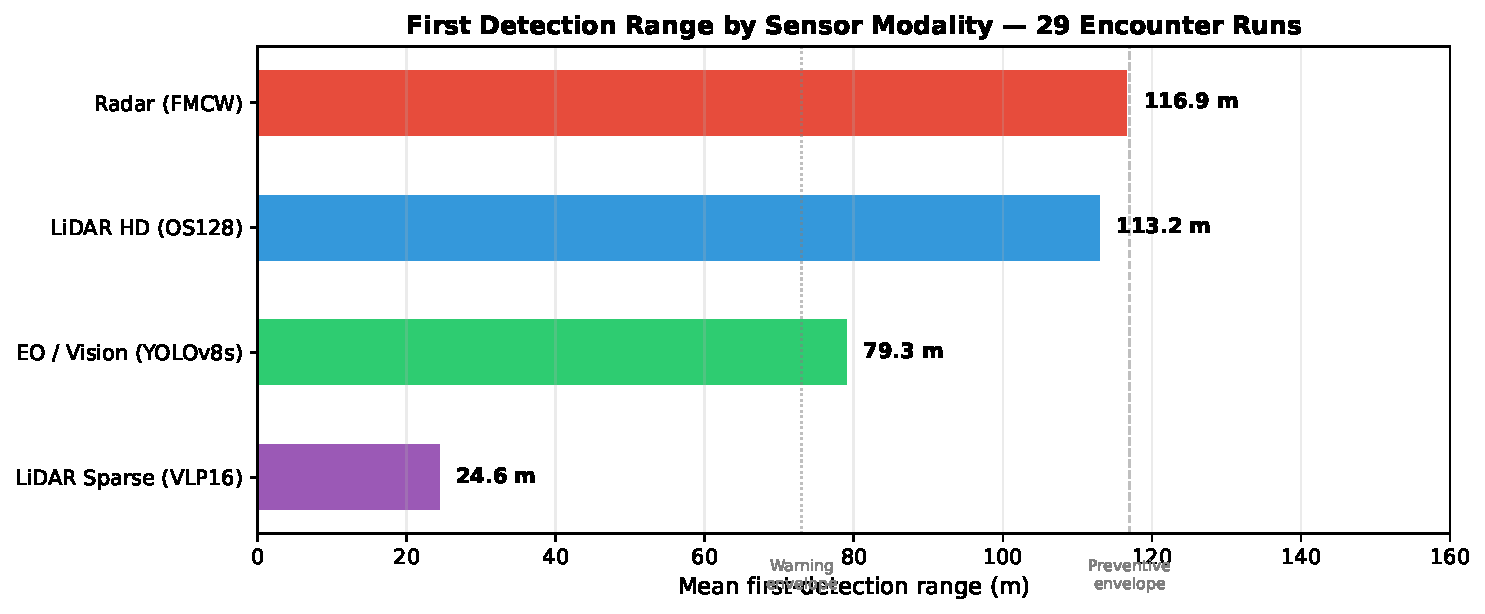
\includegraphics[width=0.95\linewidth]{figures/exp30_first_detection_range.pdf}
  \caption{Mean first-detection range by sensor modality (Radar/LiDAR: 29 runs; EO: 30 runs with trained YOLOv8s), with DAIDALUS alert-envelope reference lines. Radar provides the earliest cueing at $\sim$117\,m, followed closely by LiDAR HD; EO contributes classification at $\sim$79\,m within the Warning envelope.}
  \label{fig:first-detection}
\end{figure}

\subsubsection{Simulation Strengths and Current Limitations}

\paragraph{Validated capabilities.}
\begin{itemize}
  \item \textbf{Synchronized multi-modal acquisition}: All sensors evaluate identical encounter frames, enabling fair cross-modal comparison without temporal alignment artifacts.
  \item \textbf{Unified EO processing}: A single detection model generalizes across four distinct optical configurations (Tables~\ref{tab:eo-specialized}--\ref{tab:eo-crossval}), reducing the software certification scope for operational deployment.
  \item \textbf{Complementary detection architecture}: Radar provides the broadest coverage at all ranges, while the trained EO model now matches or exceeds LiDAR HD in the 25--100\,m operational band (91--100\% vs.\ 55--68\%). The sensors remain complementary: radar offers early warning, LiDAR provides geometric point-cloud data for spatial confirmation, and EO delivers semantic classification. This complementarity is confirmed across 30 encounter scenarios and four lighting conditions.
\end{itemize}

\paragraph{Identified limitations and required next steps.}
\begin{enumerate}
  \item \textbf{Radar classification}: The current evaluation uses return-presence detection (maximum recall) without target classification. Integrating micro-Doppler or range-profile features would enable class discrimination (drone vs.\ bird), directly reducing the nuisance alert rate analyzed in Section~2.6.4.
  \item \textbf{LiDAR clutter discrimination}: The point-cloud detector uses geometric clustering, which may produce false positives in complex urban environments. Supervised classification against static clutter is a required hardening step.
  \item \textbf{EO domain gap}: Visual training data derives from simulation segmentation. Transfer to real-world conditions (atmospheric haze, sun glare, diverse backgrounds) remains an open integration challenge requiring mixed-reality or field-collected datasets.
  \item \textbf{Encounter geometry scope}: The 30 scenarios focus predominantly on frontal and near-frontal approach geometries. Broader angular coverage, lateral intercepts, and overtaking scenarios are needed to fully characterize the sensor envelope.
  \item \textbf{No-intruder baseline}: False-alarm quantification (detections in the absence of an intruder) has not yet been conducted. This campaign is identified as a priority next step in Section~4.1.2.
\end{enumerate}

These limitations are characteristic of the current research maturity level. They define the specific hardening activities required before the simulation evidence can support higher-fidelity validation or field-test planning.

\subsubsection{Implications for the ABDAA Architecture}
\label{sec:multisensor-implications}

The empirical results from this synchronized campaign provide three specific inputs to the overall ABDAA design evaluated in this report:

\begin{enumerate}
  \item \textbf{Sensor role assignment} (feeds Section~1.2.8 architecture): Radar serves as the continuous early-warning layer with the highest availability ($P_d$ = 100\% return-presence). LiDAR HD provides geometric spatial confirmation in tactical distance bands (55--78\% detection rates from 10 to 100\,m). EO delivers semantic classification with 91--100\% reliability in the 25--100\,m operational band, with validated multi-lens generalization and a mean first-detection range of 79.3\,m.

  \item \textbf{SUM uncertainty parametrization} (feeds Section~2.4.5): The localization quality metrics from EO training (73.1\% for the unified model) quantify the spatial uncertainty that the SUM module must absorb when expanding the DAIDALUS Well Clear volume. Lower localization quality requires larger uncertainty ellipsoids, triggering earlier and more conservative avoidance maneuvers.

  \item \textbf{Environmental robustness for BVLOS operations} (feeds Section~3.2): Radar and LiDAR maintain detection capability across all lighting conditions, supporting 24-hour corridor operations. While EO performance varies by lighting (39.5\% at dawn to 65.9\% at night), it no longer exhibits complete failure under any condition --- confirming that the trained model provides meaningful contribution across the diurnal cycle. Nonetheless, the variation reinforces the hybrid radar+vision design selected for the ABDAA baseline.
\end{enumerate}

For DECEA evaluators, the practical value of this campaign is not a definitive sensor ranking, but rather a transparent, reproducible quantitative basis for understanding \emph{why} the hybrid architecture combines multiple modalities, \emph{what} each modality contributes to the detection timeline, and \emph{where} the current research boundaries lie. This evidence supports informed prioritization of future evaluation campaigns with broader scenarios, operational fidelity, and progressively stricter validation criteria aligned with ASTM F3442 and DO-365B requirements.
